% Figure 1. From Year 1 to an offer (wide). Labels: LABELS.md, Figure 1.
\def\eeprepfigure{1}
\providecommand{\eepstyledir}{../style}% repo: ../style
\input{\eepstyledir/circuitikz-preamble.tex}
% Colours, fonts, and text styles for the Get hired figures.
% Input after style/circuitikz-preamble.tex (in the repo: ../../style/circuitikz-preamble.tex).
% Define \eepdark before this file for the dark build. Same names as the resume figures,
% plus the rest of the navy palette. Crimson (eepaccent) marks one thing per figure.
\setmainfont{Newsreader}[
  BoldFont={Newsreader Bold},
  ItalicFont={Newsreader Italic},
  BoldItalicFont={Newsreader Bold Italic},
]
\usetikzlibrary{arrows.meta,calc,decorations.pathreplacing}
\ifdefined\eepdark
  \definecolor{eepink}{HTML}{ECEEF2}
  \definecolor{eeptext}{HTML}{D0D4DB}
  \definecolor{eepinktwo}{HTML}{A6AFBF}
  \definecolor{eepmute}{HTML}{8F95A0}
  \definecolor{eepsilver}{HTML}{76808F}
  \definecolor{eeprule}{HTML}{3B4352}
  \definecolor{eepwash}{HTML}{17243A}
  \definecolor{eepsunken}{HTML}{101828}
  \definecolor{eepfill}{HTML}{131C2E}
  \definecolor{eeppaper}{HTML}{0D1524}
  \definecolor{eepaccent}{HTML}{E06A5F}
  \definecolor{eepaccentsoft}{HTML}{2A1A24}
\else
  \definecolor{eepink}{HTML}{16233A}
  \definecolor{eeptext}{HTML}{232A39}
  \definecolor{eepinktwo}{HTML}{424D63}
  \definecolor{eepmute}{HTML}{5E636C}
  \definecolor{eepsilver}{HTML}{838C9A}
  \definecolor{eeprule}{HTML}{C4C8CF}
  \definecolor{eepwash}{HTML}{E7ECF3}
  \definecolor{eepsunken}{HTML}{F3F4F6}
  \definecolor{eepfill}{HTML}{FFFFFF}
  \definecolor{eeppaper}{HTML}{FBFBFC}
  \definecolor{eepaccent}{HTML}{A3201D}
  \definecolor{eepaccentsoft}{HTML}{F8ECEA}
\fi
% Draw in y-down points so coordinates read like a mockup: [x=1pt, y=-1pt].
\tikzset{
  eeptitle/.style={anchor=base west, inner sep=0pt, text=eepink, font=\rmfamily\bfseries\fontsize{26}{31}\selectfont},
  eephead/.style={inner sep=0pt, text=eepink, font=\sffamily\bfseries\fontsize{14.5}{18}\selectfont},
  eepbody/.style={inner sep=0pt, text=eepinktwo, font=\sffamily\fontsize{13}{17}\selectfont},
  eepnote/.style={inner sep=0pt, text=eepmute, font=\sffamily\fontsize{12.5}{16}\selectfont},
  eepsrc/.style={anchor=north west, inner sep=0pt, align=left, text=eepmute, font=\sffamily\fontsize{11}{14.5}\selectfont},
  eepbox/.style={draw=eepink, fill=eepfill, rounded corners=4pt},
  eepfocus/.style={draw=eepaccent, fill=eepfill, rounded corners=4pt, line width=1.8pt},
  eeparrow/.style={-{Stealth[length=8pt,width=6pt]}},
  eepdash/.style={dash pattern=on 4pt off 4pt},
  eeplead/.style={draw=eepsilver, line width=0.9pt},
}
% A dot on a trace, like a schematic junction.
\newcommand{\eepdot}[2][eepink]{\fill[#1] #2 circle (3.6pt);}
% Short labels never hyphenate.
\hyphenpenalty=10000 \exhyphenpenalty=10000
% One space after a full stop, as on the site.
\frenchspacing

\newcommand{\tlstop}[4]{% #1 x, #2 heading, #3 lines, #4 colour of heading
  \node[anchor=north west, inner sep=0pt, text width=112pt, align=left] at ({#1-4},118)
    {{\sffamily\bfseries\fontsize{13}{16}\selectfont\color{#4}#2\par}\vspace{7pt}%
     {\sffamily\fontsize{12}{15.5}\selectfont\color{eepinktwo}#3\par}};}
\newcommand{\gap}{\par\vspace{6pt}}
\begin{document}
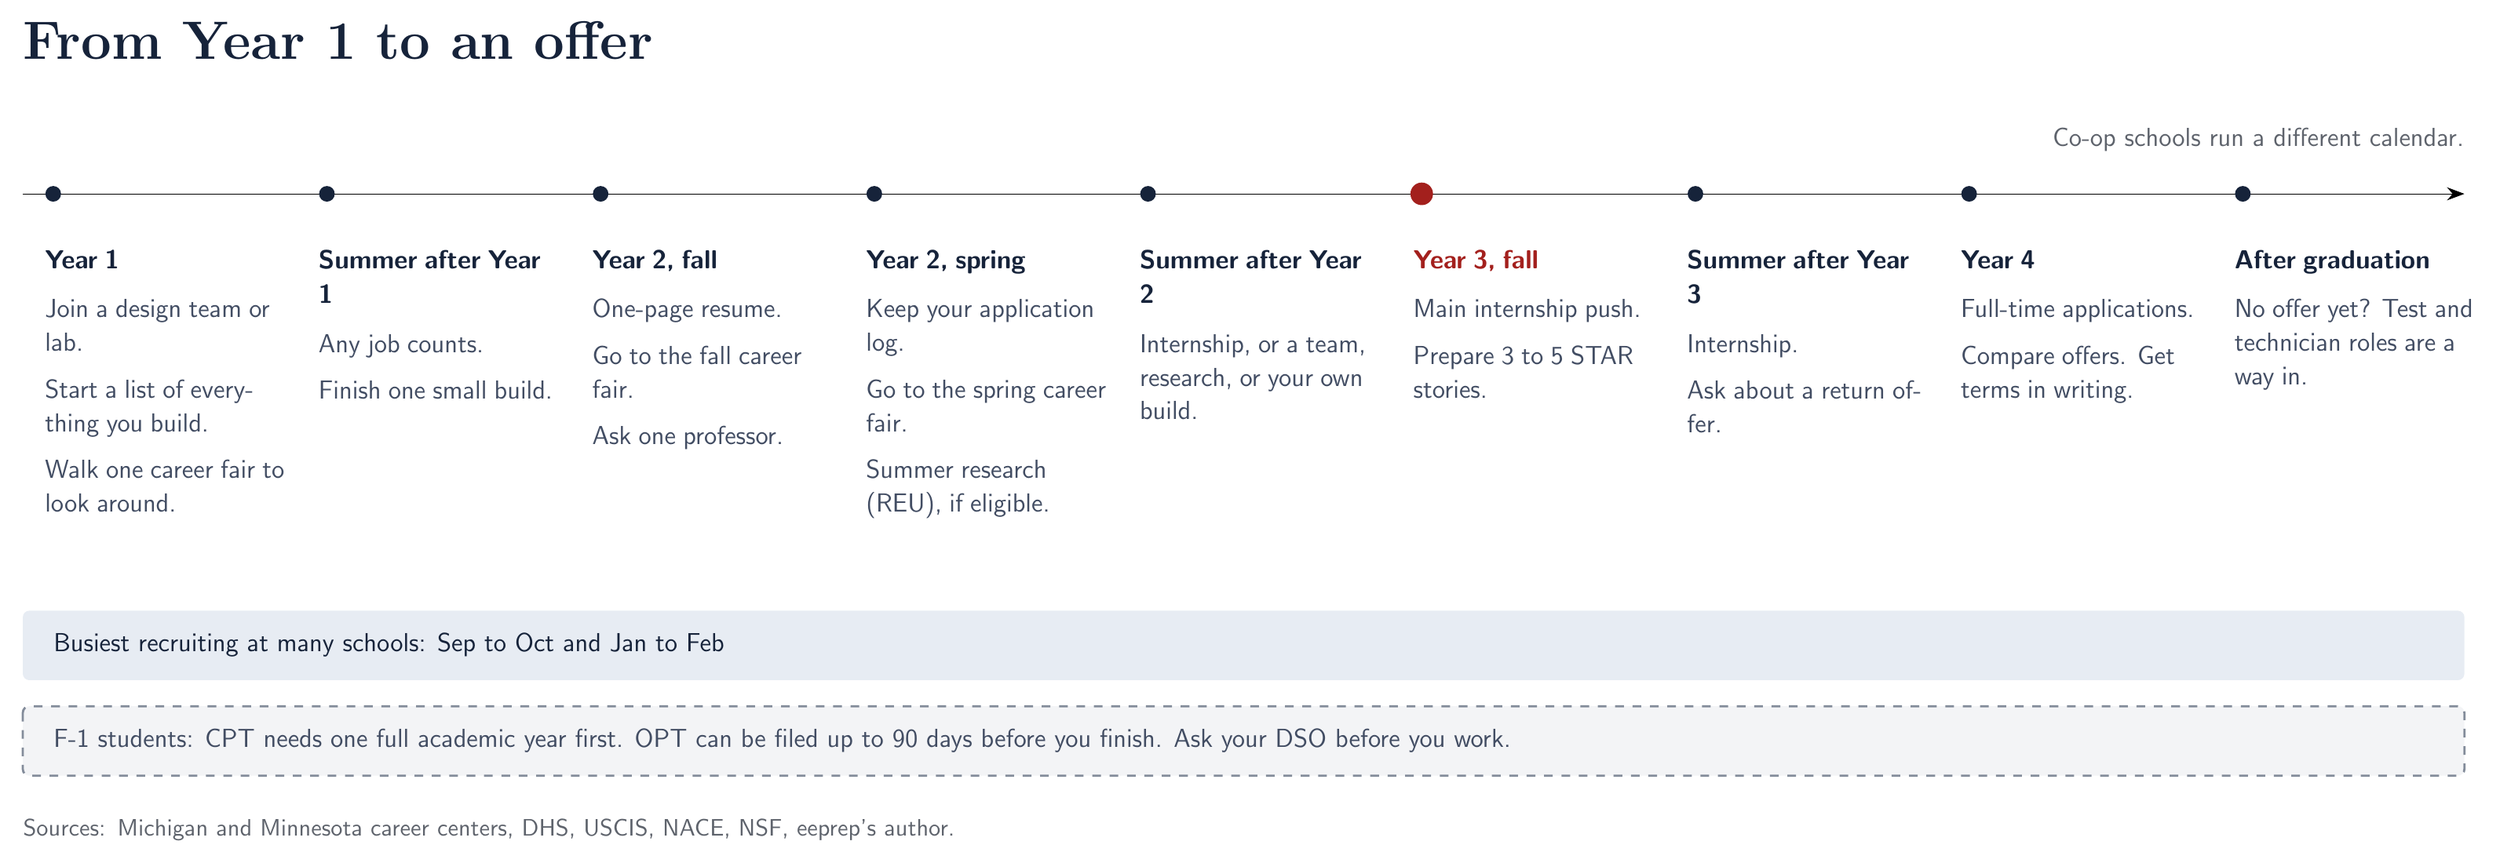
\begin{tikzpicture}[x=1pt,y=-1pt]
  \node[eeptitle] at (0,30) {From Year 1 to an offer};
  \node[eepnote, anchor=base east] at (1124,70) {Co-op schools run a different calendar.};
  % The trace: one signal line, a junction dot per stop.
  \draw[eeparrow] (0,92) -- (1124,92);
  \foreach \i in {0,...,8} { \pgfmathsetmacro\x{14+\i*126} \ifnum\i=5\else\eepdot{(\x,92)}\fi }
  \fill[eepaccent] (644,92) circle (5.2pt);
  \tlstop{14}{Year 1}{Join a design team or lab.\gap Start a list of everything you build.\gap Walk one career fair to look around.}{eepink}
  \tlstop{140}{Summer after Year 1}{Any job counts.\gap Finish one small build.}{eepink}
  \tlstop{266}{Year 2, fall}{One-page resume.\gap Go to the fall career fair.\gap Ask one professor.}{eepink}
  \tlstop{392}{Year 2, spring}{Keep your application log.\gap Go to the spring career fair.\gap Summer research (REU), if eligible.}{eepink}
  \tlstop{518}{Summer after Year 2}{Internship, or a team, research, or your own build.}{eepink}
  \tlstop{644}{Year 3, fall}{Main internship push.\gap Prepare 3 to 5 STAR stories.}{eepaccent}
  \tlstop{770}{Summer after Year 3}{Internship.\gap Ask about a return offer.}{eepink}
  \tlstop{896}{Year 4}{Full-time applications.\gap Compare offers. Get terms in writing.}{eepink}
  \tlstop{1022}{After graduation}{No offer yet? Test and technician roles are a way in.}{eepink}
  % Two bands under the line, across every year.
  \fill[eepwash, rounded corners=3pt] (0,284) rectangle (1124,316);
  \node[eepbody, anchor=west, text=eepink] at (14,300) {Busiest recruiting at many schools: Sep to Oct and Jan to Feb};
  \draw[eepsilver, line width=1pt, eepdash, fill=eepsunken, rounded corners=3pt] (0,328) rectangle (1124,360);
  \node[eepbody, anchor=west] at (14,344) {F-1 students: CPT needs one full academic year first. OPT can be filed up to 90 days before you finish. Ask your DSO before you work.};
  \node[eepsrc, text width=1124pt] at (0,380) {Sources: Michigan and Minnesota career centers, DHS, USCIS, NACE, NSF, eeprep's author.};
\end{tikzpicture}
\end{document}
